\section{Introdução}
Nesta secção é apresentado  o trabalho desenvolvido em cada um dos projectos realizados durante o estágio do Mestrado. À semelhança do capítulo anterior, o desenvolvimento de cada projecto é descrito num subcapítulo dedicado.



\section{Coletor de dados - Nidus} 
\par Durante o estágio o projeto referente ao coletor de dados Nidus apresenta 5 subsecções a tratar: 1) o desenvolvimento do sistema de tradução para a página do equipamento no menor espaço de memória possível; 2) a compressão dos ficheiros; 3) compressão de imagens de modo a melhorar/manter a página com layouts e funcionalidades de acordo com a concorrência e atualidade; 4) o desenvolvimento de páginas com layouts específicos; 5) a correção de \textit{Bug's} que possam existir e venham a ser descobertos. Cada um dessas subsecções serão abordadas em cada subsecção seguinte.

\subsection{Sistema de tradução automática}\label{myi18n}
\par Os sistemas de internacionalização das páginas web, fornecem ao utilizador final um sistema com tradução automática para a língua pretendida, são cada vez mais utilizados. Isto acarreta um acréscimo da complexidade do sistema e por consequência o acréscimo do escaço ocupado pelo código. O sistema utilizado no caso particular das páginas web com JavaScript é o I18N, uma \textit{Framework} desenvolvida em JavaScript, com várias funcionalidades além da tradução de páginas, tais como por exemplo a plurarização das traduções, carregamento dinâmico dos dicionários por ajax entre outros. Estas funcionalidades extras não necessárias para o projeto apenas acarretam o aumento do peso do plugin no sistema, diminuindo possibilidades futuras de alterações e novos desenvolvimentos. Para tal será desenvolvido de raiz um sistema similar ao I18N apenas com as funcionalidades pretendias de modo a ser possível comparar a diferença de espaço ocupado.


\subsubsection{O funcionamento}
\par Os sistemas de tradução são baseados numa função chamada no momento necessário da obtenção de uma tradução onde é passado um parâmetro indicando qual a tradução pretendida. Esta função é responsável por percorrer o conjunto de traduções da língua selecionada e através de um sistema associativo chave-valor retornar caso este exista o valor para a chave fornecida. Caso este não exista é devolvido o valor \textit{default}, por norma a chave do mesmo. Na figura \ref{i18n} é apresentado o esquema do funcionamento do sistema de tradução descrito acima.

\begin{figure}[ht]
\centering
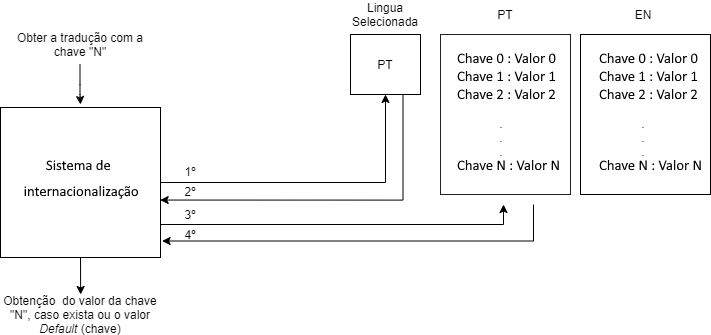
\includegraphics[width=0.95\textwidth]{images/i18n.png}
\caption{Processo da obtenção da tradução de um valor}\label{i18n}
\end{figure}

\par Após análise as funcionalidades requeridas para o projeto Nidus, são as seguintes:

\begin{itemize}
\item Tradução automática da página
\item Armazenamento persistente da linguagem escolhida
\item Alteração da linguagem pretendida, mediante a lista de opções
\item Carregamento das linguagens dinamicamente.
\end{itemize} 

\par De modo a armazenar a linguagem selecionada pelo utilizador, esta estará alocada no browser sob a forma de uma \textit{cookie}. No momento de uma tradução, o sistema verifica o valor da \textit{cookie} em vigor e procura na associação chave-valor respetiva á linguagem selecionada, se a chave pretendida existe e caso exista o valor desta é devolvida. Caso a \textit{cookie} não exista é devolvida a opção \textit{default}.

\par O Sistema é composto por 4 funções. A primeira, gLng, responsável por verificar se existe a \textit{cookie} no \textit{browser} e retornar o seu valor ou o valor da língua \textit{default}, o Inglês ("EN"). A segunda função, sLng, é utilizada aquando do guardar da linguagem para posterior utilização, esta como parâmetros recebe o valor a inserir, esta \textit{cookie} fica disponível no \textit{browser} durante 365 dias após a sua última atualização. Após guardar a \textit{cookie}, a página é recarregada de modo a atualizar todos os campos e não apenas os gerados a partir do momento da seleção da nova língua, garantindo assim que a página tenha várias línguas no mesmo instante de tempo visto que o código HTML da mesma é gerado no momento em que é necessário pelo JavaScript e é incorporado no HTML principal. A terceira função "\_" é responsável por retornar o valor da chave fornecida no único parâmetro da mesma. Caso a chave não exista na língua selecionada pela \textit{cookie} é retornado o valor de \textit{default}, correspondente á chave fornecida como parâmetro da função. Por último existe a função "ll" com dois parâmetros, como primeiro parâmetro temos a \textit{string} correspondente ás iniciais da língua a adicionar (Exemplo: "PT","EN","ES","FR") e o segundo parâmetro um objeto com associações chave-valor para a língua fornecida. Esta função é responsável por adicionar ao conjunto de dicionários a língua pretendida ou atualizar o dicionário da língua caso este já exista.
\par O conjunto de dicionários armazenado segue o esquema apresentado na figura \ref{dicextr}. No caso de apenas se pretender desenvolver numa língua é possível apenas fazer a definição das funções e não fornecer nenhum dicionário, visto nesse caso ele devolver a chave, bastando para isso a chave corresponder á tradução pretendida na única língua disponível, deixando o produto já preparado para futura implementação do sistema de internacionalização.



\begin{figure}[ht]
\centering
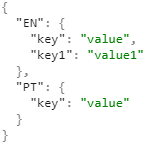
\includegraphics[width=0.25\textwidth]{images/extrjson.png}
\caption{Estrutura JSON do conjunto de dicionários}\label{dicextr}
\end{figure}

\par No excerto \ref{i19n} é apresentado o código referente ás funções criadas para o sistema.

\begin{lstlisting}[caption=Definição do Sistema de Internacionalização,label={i19n},language=JavaScript]

var _d={}; //Dicionarios

function gLng() {
	var v = document.cookie.match('(^|;) ?locale=([^;]*)(;|$)');
    return v ? v[2].toUpperCase(): "EN";
}

function sLng(v) {
    var d = new Date;
    d.setTime(d.getTime() + 31536000000);
    document.cookie ="locale=" + v + ";path=/;expires=" + d.toGMTString();
    location.reload();
}

function _(k){
    if(_d==null|| _d==undefined || cd==undefined || cd==null || _d[gLng()]==null || _d[gLng()]==undefined) {return k;}
    return _d[gLng()][k];
}

function ll(a,b){
    if(_d==null|| _d==undefined){ _d={};}
    _d[a]=b;
}
\end{lstlisting}



\subsubsection{Resultados obtidos}
\par Após comparação do sistema implementado em comparação com o I18N\cite{i18n} é possível observar a redução do tamanho para cerca de 34 \% ( 1178b - 66\% = 404b), este valor foi obtido na comparação entre as duas versões minificadas e comprimidas com o GZIP como é possível observar no gráfico apresentado na figura \ref{garph1}, no gráfico é possível verificar os tamanhos originais, após a minificação e o tamanho do minificado após a compressão com o GZIP. Ambos valores relativos à comparação não contemplam os dicionários, apenas o código inerente á utilização das funcionalidades.

\begin{figure}[ht]
\centering
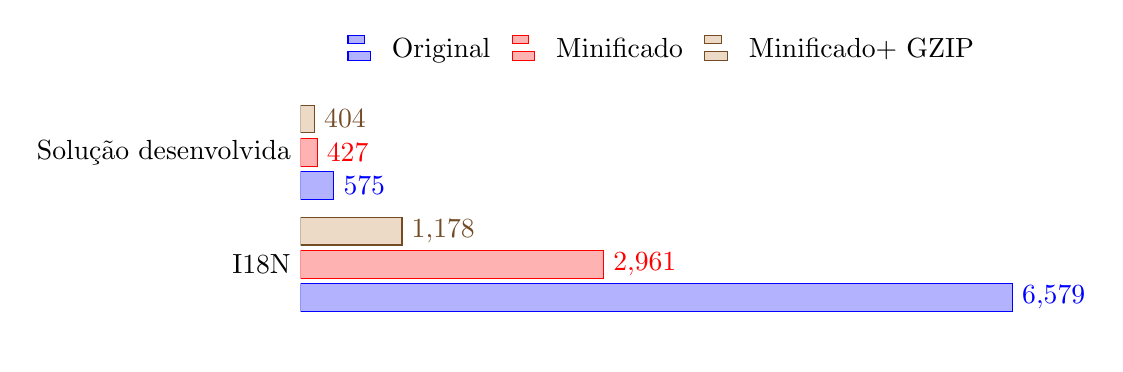
\begin{tikzpicture}
\begin{axis}[
xbar,
height=5cm,width=10.8cm, 
y axis line style = { opacity = 0 },
axis x line = none,
tickwidth = 0pt,
enlarge y limits = 0.7, 
enlarge x limits = 0.02,
symbolic y coords = {I18N, Solução desenvolvida},
nodes near coords,
ytick=data,
legend style={
at={(rel axis cs:0.5,1)},
anchor=south,
legend columns=-1, 
column sep=2mm, 
draw=none 
}
]
\addplot coordinates { (6579,I18N) (575,Solução desenvolvida) };
\addplot coordinates { (2961,I18N) (427,Solução desenvolvida) };
\addplot coordinates { (1178,I18N) (404,Solução desenvolvida) };
\legend{Original, Minificado, Minificado+ GZIP}
\end{axis}
\end{tikzpicture}

\caption{Gráfico com comparação do tamanho entre versões (em Bytes)}\label{garph1}
\end{figure}

\subsection{Compressão de ficheiros}\label{compress1}

\par Durante o estágio foi estudado igualmente a comparação entre a utilização do GZIP e do Brotli de modo a analisar as vantagens e desvantagens aplicadas ao projeto em questão.
\par Segundo estudos online \cite{brotlivsgzip}, é possível analisar que comparando apenas o Brotli e o GZIP, que este último tem uma taxa de compressão inferior, significa isto que o mesmo ficheiro após compressão é maior no caso do GZIP, tornando o Brotli um candidato a ponderar. Já no campo da velocidade de descompressão o caso inverte, sendo o GZIP a possuir melhores resultados, este parâmetro, não afeta o espaço ocupado na memória do microcontrolador. A velocidade de compressão é inferior no Brotli não o tornando ideal para compressões em tempo real, mas visto o servidor WEB alojado na Nidus já possuir todos os ficheiros comprimidos e estes são sempre estáticos, o tempo de compressão não afeta o equipamento neste projeto. 
\par Visto o método Brotli possuir mais valias ao projeto, de modo a estudar e comparar as vantagens/desvantagens inerentes á migração para o Brotli, serão comprimidos os ficheiros atuais do projeto em ambos os métodos de modo a analisar os ganhos obtidos no projeto em especifico antes da sua atualização. Na tabela \ref{tabw2} são apresentados os resultados obtidos para cada ficheiro do projeto, os valores apresentados correspondem ao tamanho em bytes. No valor apresentado correspondente ao tamanho original, este no caso do HTML e CSS encontra-se minificado, caso seja JavaScript este encontra-se minificado e comprimido com recurso ao Google Clousure Compiler.


\begin{table}[htb]
\caption{Comparação entre Brotli e GZIP}\label{tabw2}
\begin{tabular}{|c|c|c|c|c|}\hline
Tipo do Ficheiro& \begin{tabular}{@{}c@{}} Tamanho original\\ Minificado\end{tabular} &Tamanho GZIP& Tamanho Brotli& Diferença \\\hline
JavaScript&230 304 & 58 061&52 453& -5 608 \\\hline
JavaScript&462 316& 95 196& 75 702& -19 494\\\hline
JavaScript&627 032& 221 754&206 150& -15 604 \\\hline
JavaScript&140 389 & 46 945& 42 687&-4 258\\\hline
JavaScript&84 249 & 28 579&26 594&-1 985\\\hline
HTML&37 302 & 16 728& 15 893&-835\\\hline
HTML&39 352 & 17 251& 16 348&-903\\\hline
FONT (.TTF)&111 368 & 66 831&62 819&-4 012\\\hline
CSS&53 642 & 6 815& 5 956&-859\\\hline
CSS&100 495 & 15 524&12 826&-2 698\\\hline
CSS&49 145 & 5 674&4 771&-903\\\hline
FAVICON&1150& 352&348&-4\\\hline
Total&1 936 744&579 710&522 547&-57 163\\\hline
\end{tabular} 
\end{table}

\par Analisando os ganhos obtidos com a utilização do Brotli é possível libertar cerca de 57 KB alterando o método de compressão dos ficheiros. De modo a realizar a migração entre a utilização do GZIP e Brolti apenas é necessário alterar o \textit{software} desenvolvido responsável por comprimir os ficheiros originais na sua respetiva compressão de forma autónoma e a alteração dos cabeçalhos enviados pelo servidor aquando de uma resposta por parte deste para o cliente. Na figura \ref{packet123} é possível observar a diferença presente nos cabeçalhos da resposta HTTP proveniente do \textit{browser}.
\par Estas fases não serão realizadas durante o estágio referente deste relatório.

\begin{figure}[ht]
\centering
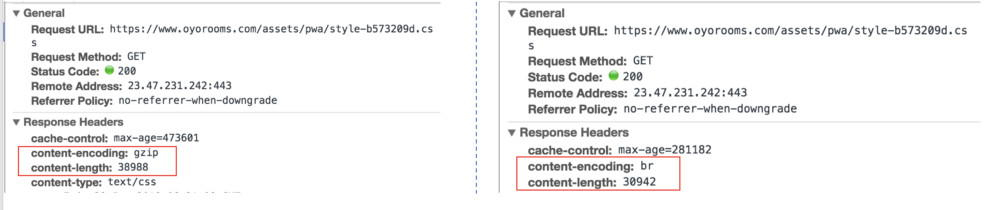
\includegraphics[width=0.95\textwidth]{images/header.png}
\caption{Comparção entre os \textit{headers} HTTP GZIP e Brotli\cite{headerImage}}\label{packet123}
\end{figure}


\subsection{Compressão de imagens}\label{compressimaage}

\par As imagens são um ponto importante dos sistemas IOT, onde o utilizador através de esquemas, imagens e gráficos consegue obter o que pretende sem muito esforço. O sistema Nidus apenas despõe de imagens em algumas versões a pedido de clientes devido ao sobre carregamento de espaço que acarreta a utilização de imagens.
\par Para desenvolver uma interface com recurso a sistemas visuais é necessário ter ou uma imagem com uma qualidade estipulada para o ecrã máximo necessário para ser possível reduzir a mesma em ecrãs mais pequenos, ou existirem múltiplas imagens de vários tamanhos para cada tipo de ecrã. A utilização de imagens pequenas que ocupem pouco espaço em disco, aquando da utilização em ecrãs maiores irá deixar visível na imagem cada pixel revelando ao utilizador a fraca qualidade do sistema. Na utilização de imagens superior ao máximo dos ecrãs e fazer o redimensionamento para um tamanho inferior, torna as imagens mais atrativas, pois o efeito não provoca o aparecimento da imagem “Pixelizada”. Isto implica mais espaço de memória para alojar imagens, que não existe na configuração de \textit{hardware} atual do sistema Nidus. Em alternativa às codificações mais comuns nas imagens (PNG, JPEG, entre outras) existe a possibilidade de em imagens que não representem fotografias a utilização de SVG. No SVG ao contrário dos outros formatos indicados não é feita a representação de cada pixel da imagem, mas sim a definição de uma função que representa uma reta, uma forma, um polígono, ou as coordenadas de pontos, sobre a forma de uma estrutura XML. O HTML já possui suporte  para elementos SVG, Na utilização de SVG dentro de páginas HTML é possível a utilização de todas as funcionalidades inerentes ao CSS tais como criar animações. 
\par Outra funcionalidade possível com a utilização de SVG é a alteração do texto existente na imagem apenas fazendo a alteração do valor do elemento XML, à semelhança da alteração do texto numa página HTML.

\par Os editores de SVG possuem variadas opções que não representam nada para o utilizador final, são apenas informações para o próprio editor. Para remover essa informação são utilizadas ferramentas para a remoção de tal informação. A ferramenta escolhida durante o estágio foi a SVGO\cite{svgo}, uma ferramenta desenvolvida em node.js que permite otimizar os SVG. Com esta ferramenta é possível remover toda a informação desnecessária e otimizar e simplificar algumas funções não afetando a qualidade da imagem. De modo a ser possível em tempo real fazer alterações é necessário, à semelhança das páginas HTML, cada elemento possuir um ID para fazer a sua procura na árvore XML e deste modo ser possível alterar a cor, o conteúdo do texto adicionar animações. O próprio SVG possibilita a inserção de imagens PNG, JPEG dentro do SVG. Estas imagens são adicionadas ao XML sob a forma de Base64. No apêndice \ref{svg} é apresentado o exemplo do SVG gerado pelo editor. No Apêndice \ref{svggo} a respetiva compressão utilizando a ferramenta SVGO. Uma das considerações na utilização do SVGO é a necessidade de preservar os ID's e não os remover durante a compressão. Para tal na utilização da ferramenta é necessário indicar que  pretendemos manter os ID's, para tal basta durante a utilização utilizar a opção '--disable=cleanupIDs'.

\par Para criar animações á semelhança do HTML é possível atribuir classes a cada elemento do SVG e tirar partido das animações possíveis no CSS. 
\par No gráfico da figura \ref{compSV} é apresentado o tamanho ganho na compressão do SVG do Apêndice \ref{svg}. O Tamanho do SVG após a otimização com a ferramenta SVGO é de apenas cerca de 20\% do tamanho original (2 485b - 80\%= 559b).

\begin{figure}[ht]
\centering
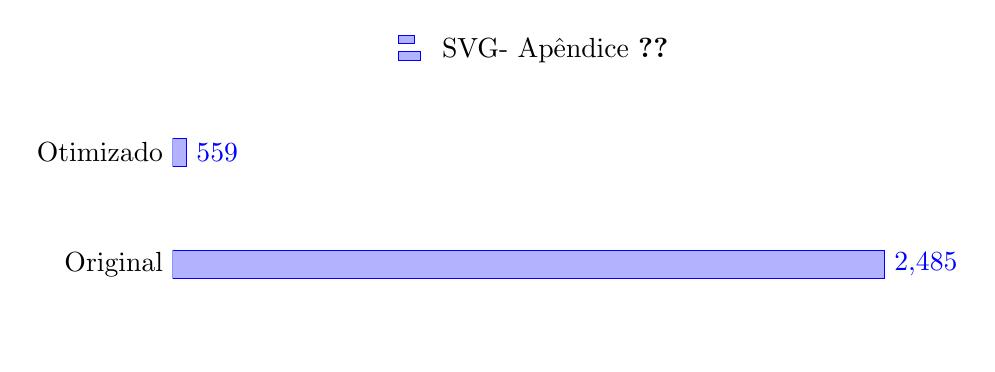
\begin{tikzpicture}
\begin{axis}[
xbar,
height=5cm,width=10.8cm, 
y axis line style = { opacity = 0 },
axis x line = none,
tickwidth = 0pt,
enlarge y limits = 0.7, 
enlarge x limits = 0.02,
symbolic y coords = {Original, Otimizado},
nodes near coords,
ytick=data,
legend style={
at={(rel axis cs:0.5,1)},
anchor=south,
legend columns=-1, 
column sep=2mm, 
draw=none 
}
]
\addplot coordinates { (2485,Original) (559,Otimizado) };
\legend{SVG- Apêndice \ref{svg}}
\end{axis}
\end{tikzpicture}

\caption{Gráfico com comparação do tamanho entre original e otimizado(em Bytes)}\label{compSV}


\end{figure}

\subsection{Desenvolvimento a pedido de cliente}\label{custom}

\par Durante o estágio existiu apenas um desenvolvimento pedido pelo cliente. O cliente pretende utilizar uma Nidus IT para controlar o seu sistema de alimentação dos animais de forma automática. Além de todas as questões a tratar no Back-end da Nidus, relativas a funcionamentos específicos da solução, o cliente pretende aceder na página da Nidus uma interface visual para inserir num monitor com o estado da alimentação, dos motores, da água. Este desenvolvimento para a sua realização usou as capacidades referidas no capítulo \ref{compressimaage}, de modo para obter uma imagem única e responsiva com animações em tempo real. Após o desenho da interface pretendida no editor SVG, o mesmo foi comprimido com a ferramenta SVGO indicada anteriormente. \par De modo a criar uma interface atrativa ao utilizador foram criadas algumas animações nas linhas de alimentação, no silo da alimentação indicando o seu estado atual visualmente e numéricamente, tal como o estado das condutas de água.

\begin{figure}[ht]
\centering
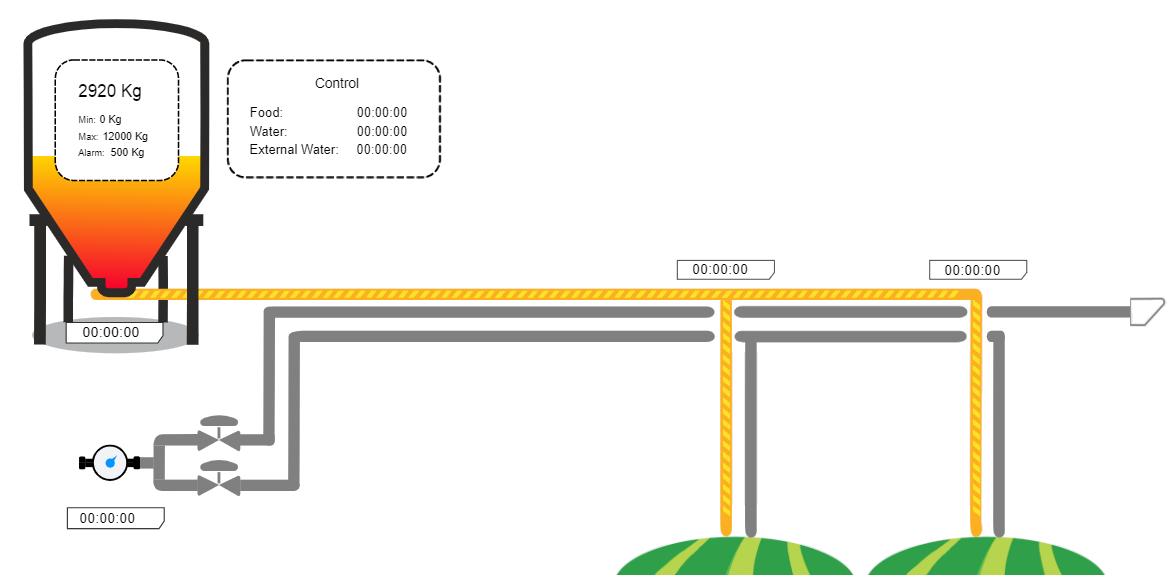
\includegraphics[width=0.95\textwidth]{images/svgpig.png}
\caption{Exemplo do SVG utilizado na Solução}\label{pig}
\end{figure}

\subsection{Correção de \textit{bugs}}\label{Bug}

\par Durante o estágio apenas foi reportado a existência de um \textit{bug}. Estre prede-se com a estrutura criada para comunicação entre o \textit{Front-end} e o \textit{Back-end} ou com sistemas que pretendam integrar os equipamentos Nidus.
\par No momento do carregamento da página WEB, a mesma solicita um ficheiro XML com todas as informações necessárias. Em alguns dos pontos da estrutura como por exemplo o caso dos Input, Outputs, Sensores, entre outros, os mesmos são agrupados num elemento principal como é possível observar no exemplo \ref{xml1}.


\begin{lstlisting}[caption=Estrutura parcial do XML da Nidus(Sensores),label={xml1},language=XML]
...
<Sensors>
    <Entry>
        <ID>0</ID>
...
    </Entry>
    <Entry>
        <ID>1</ID>
...
    </Entry>
...
</Sensors>
\end{lstlisting}




\par Este ID é utilizado na comunicação de modo a indicar a que sensor se refere os dados. O problema surge aquando da eliminação de um sensor. Supondo o seguinte cenário. O Utilizaodr elimina na página o sensor com o ID 0, o sistema Nidus elimina o sensor e a entrada no XML com o ID 0 fica inutilizada passado o XML a conter os ID's 1,2,3,4 ,... de modo ao sistemas que integram a Nidus poderem utilizar o ID como um identificador único. O problema reside no código JavaScript que converte o XML numa variável JavaScript, mais concretamente num \textit{array}. O sistema em alguns dos pontos do código ao invés de utilizar o valor presente no elemento ID, utilizava a sua posição no \textit{array}, fazendo que em sistemas onde tivessem sido feitas alterações (Exemplo: eliminar sensores) os ID's não correspondiam. Supondo o exemplo \ref{xml2} onde existem dois sensores com os ID's 0 e 1. Na conversão para um objeto no JavaScript era obtida a estrutura apresentada na figura \ref{estruct1}.

\begin{lstlisting}[caption=Exemplo do XML antes da eliminação de Sensores,label={xml2},language=XML]
...
<Sensors>
    <Entry>
        <ID>0</ID>
        <Name>0</Name>
    </Entry>
    <Entry>
        <ID>1</ID>
        <Name>1</Name>
    </Entry>
</Sensors>
...
\end{lstlisting}

\begin{figure}[ht]
\centering
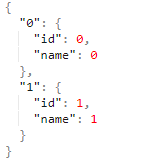
\includegraphics[width=0.25\textwidth]{images/estructu1.png}
\caption{Estrutura obtida no JavaScript - 1}\label{estruct1}
\end{figure}

\par Após a eliminação do Sensor 0, o XML obtido é similar ao apresentado no código \ref{xml3}. Neste caso o \textit{array} criado no JavaScript era similar ao apresentado na figura \ref{estruct2}. O problema reside na utilização da posição do \textit{array} em algumas partes do código nomeadamente na procura do sensor. No exemplo apresentado na figura \ref{estruct2} antes da correção do \textit{bug} o código existente ao necessitar dos dados do sensor com o ID 1 aceder á posição 1 do \textit{array}, ao invés de procurar por cada elemento qual o elemento que possui aquele id. 
\par No caso de terem sido eliminados alguns sensores como apresentado exemplo \ref{xml3} os dados selecionados não correspondem ao pretendido pelo utilizador e apresentados na página de configurações. Os valores apresentados na página inicial, onde são mostrados os valores em tempo real e o mínimo e máximo do sensor não possuiam este Bug estando limitado á alguma configurações dos sensores e a criação de Eventos.

\begin{lstlisting}[caption=Exemplo do XML após eliminação do Sensor,label={xml3},language=XML]
...
<Sensors>
    <Entry>
        <ID>1</ID>
        <Name>1</Name>
    </Entry>
    <Entry>
        <ID>2</ID>
        <Name>2</Name>
    </Entry>
</Sensors>
...
\end{lstlisting}

\begin{figure}[ht]
\centering
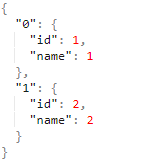
\includegraphics[width=0.25\textwidth]{images/estruct2.png}
\caption{Estrutura obtida no JavaScript - 2}\label{estruct2}
\end{figure}


\par De modo a resolver o problema identificado foi criada no projeto uma função findObjectByKey, apresentada no exemplo \ref{js2}, com 3 parâmetros. No primeiro parâmetro é indicado o \textit{array} onde deve o sistema procurar. Em seguida é indicado em que propriedade pretendemos compara e por último indicamos o valor que pretendemos encontrar. No código seguinte é apresentado o código utilizado. Caso o elemento não exista é devolvido o valor \textit{null}.

\begin{lstlisting}[caption=Função findObjectByKey,label={js2},language=JavaScript]
function findObjectByKey(array, key, value) {
    for (var i = 0; i < array.length; i++) {
        if (array[i][key].toString() === value.toString()) {
           return array[i];
        }
    }
    return null;
}
\end{lstlisting}

\par Para a correção deste \textit{Bug} é necessário analizar todo o código e ao invés do acesso á posição diretamente no \textit{array} é necessário a alteração de todo o código para fazer utilização da função e obter o valor correto.


\subsection{Melhoramento da página}
\par Após análise prévia da página do sistema Nidus, foi acordado a necessidade de desenvolver um sistema mais simplificado para o processo de criação de eventos. Pretende-se assim estudar a melhor solução para a criação das ações e das reações e uma interface para criar os eventos com recurso às ações e reações previamente criadas. Todas as opções e menus para a criação e manutenção das ações e reações mantém-se inalteradas no momento atual. Já a criação de eventos necessita de ser restruturado, após debate chegou-se á decisão de necessitar de um sistema visual onde o utilizador por blocos é capaz de criar a situação que pretende.
\par Durante o estágio foram analisadas as opções possíveis para a solução pretendida. Após análise foi adotado a utilização do plugin Blockly\cite{blockly}, devido á sua semelhança com o pretendido (Scratch) e devido ao baixo espaço ocupado pós compressão e à possibilidade de criar os próprios tipos de blocos. Devido aos restantes projetos realizados durante o estágio este desenvolvimento ainda não se encontra concretizado e apenas foi selecionado a solução a adotar. No gráfico da Figura \ref{block} é apresentado o espaço ocupado pelo código fonte do \textit{plugin} escolhido.


\begin{figure}[ht]
\centering
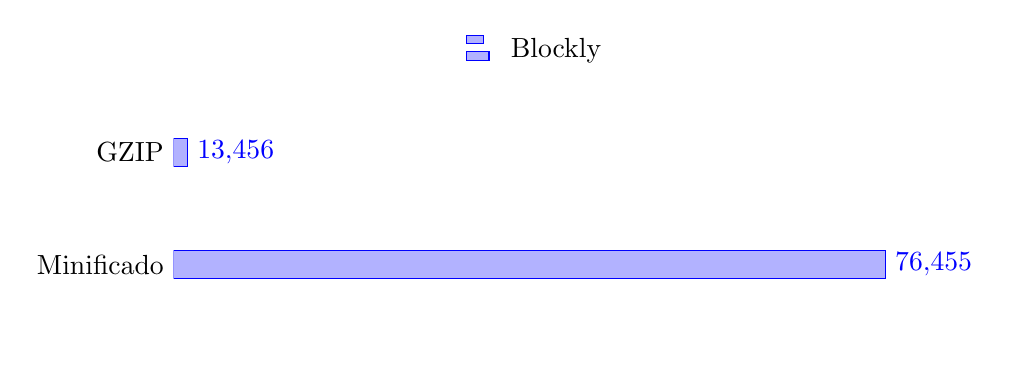
\begin{tikzpicture}
\begin{axis}[
xbar,
height=5cm,width=10.8cm, 
y axis line style = { opacity = 0 },
axis x line = none,
tickwidth = 0pt,
enlarge y limits = 0.7, 
enlarge x limits = 0.02,
symbolic y coords = {Minificado, GZIP},
nodes near coords,
ytick=data,
legend style={
at={(rel axis cs:0.5,1)},
anchor=south,
legend columns=-1, 
column sep=2mm, 
draw=none 
}
]
\addplot coordinates { (76455,Minificado) (13456,GZIP) };
\legend{Blockly}
\end{axis}
\end{tikzpicture}

\caption{Gráfico com comparação do tamanho do plugin Blockly (em Bytes)}\label{block}


\end{figure}



\section {NB-Iot \& Digi Xbee 3 }
\par
O desenvolvimento do projeto NB-Iot \& Digi Xbee 3 é composto por 4 fases, 3 das quais desenvolvidas durante este estágio. A fase não desenvolvida durante o estágio refere-se ao desenho e produção do \textit{hardware} e a parte do \textit{software} referente á leitura de sensores (comunicação entre \textit{hardware} desenvolvido e \textit{software}). As fases realizadas durante o estágio são a implementação do envio do pacote definido com os mecanismos de proteção e segurança, sincronismo dos tempos de leitura e envio e testes ao sistema.

\subsection {Envio de dados para o portal}

\par Como foi indicado no Capítulo \ref{nbiot} a estrutura de pacote a enviar é similar ao do outro produto desenvolvido pela Captemp. Este pacote é enviado através de um pacote UDP para o portal que posteriormente confirma a receção na camada de aplicação. O tamanho máximo definido para este pacote é de 1000 bytes.
A estrutura criada pela Captemp segue o formato apresentado na figura \ref{packet}.
\par No primeiro cabeçalho é possível obter os dados do equipamento que fez o envio tais como a data de envio, o IMEI, a versão do mesmo e o CRC do pacote para confirmar a integridade do mesmo. No restante do pacote são adicionados vários sub pacotes seguindo a estrutura apresentada na figura \ref {packet}, o primeiro byte indica o tipo de dados se é o envio do valor de um sensor, ou  uma configuração do equipamento(Exemplo: Operadora), o byte seguinte fornece o número de bytes dos dados e posteriormente segundo o número de bytes, o valor (Exemplo: operadora ="ALTICE").

\begin{figure}[ht]
\centering
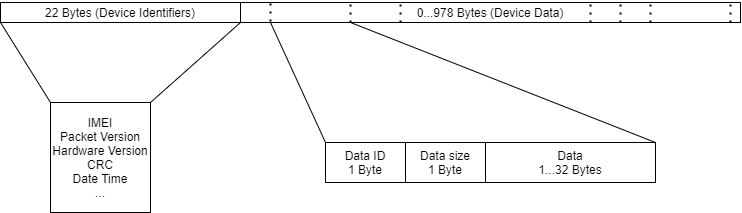
\includegraphics[width=0.95\textwidth]{images/packetnb.png}
\caption{Estrutura do Pacote NB-IOT}\label{packet}
\end{figure}

\subsection {Gestão de memória}

\par O principal motivo da desistência da utilização deste equipamento como o equipamento principal da Captemp para o NB-Iot prendeu-se com a incorreta gestão de memória do MicroPython. Segundo a documentação, quando uma variável já não é acessível pelo código o espaço ocupado em memória por esta é libertado pelo \textit{Garbage Collector} mas o espaço libertado nem sempre consegue ser reutilizador pelo MicroPython futuramente e este realiza a alocação no final ao invés de procurar o primeiro espaço disponível. No esquema apresentado na figura \ref{memo} é apresentado o comportamento da memória com a gestão nativa do MicroPython, com o decorrer do tempo a memória fica totalmente alocada não permitindo ao equipamento guardar novas leituras nem enviar para o portal.


\begin{figure}[ht]
\centering
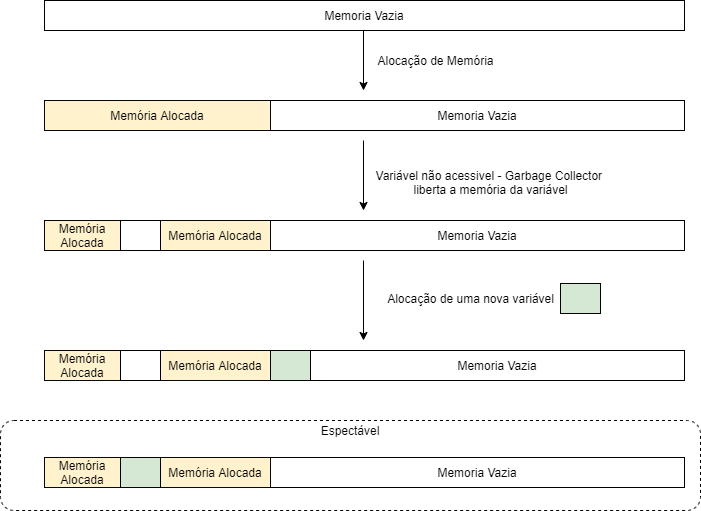
\includegraphics[width=0.90\textwidth]{images/memo.png}
\caption{Comportamento da gestão de Memória do MicroPython}\label{memo}
\end{figure}



\subsubsection {Diminuição da alocação de memória}

\par A modo de resolver a incorreta gestão de memória é necessário diminuir a alocação de novas variáveis. Para tal todo o código do programa possui todos os dados necessário em constantes e buffers de tamanhos fixos as quais nunca são eliminados ou alocam memória para mudar de tamanho, apenas alteram o seu valor. Os dois pontos críticos identificados são o \textit{array}  circular com as leituras dos sensores e a criação do pacote de envio para o portal \textit{Cloud}.
\par Na criação do pacote todos os cabeçalhos fixos são alocados em constantes globais que não vem o seu valor alterado não afetando a memória e os valores que podem ser alterados são guardados em \textit{buffers} globais criados no inicio e tem o seu tamanho estático. Devido á utilização de um módulo que não possui suporte para \textit{multi thread}, não existe problema de sincronismo entre os fluxos ao utilizar as variáveis e os \textit{buffers} globais. Ao recolher um dado de modo a enviar para o portal, como por exemplo a operadora, este tem de ser alocado num \textit{buffer} que depois é enviado pela rede para o servidor. Este \textit{buffer} de bytes, com o tamanho fixo do máximo do pacote de envio, é utilizado para fazer a concatenação dos vários campos antes do envio ao invés da abordagem anterior da utilização de um \textit{buffer} de tamanho dinâmico. Caso se pretenda adicionar valores a enviar é consultada o ultimo \textit{byte} ocupado, encontrado numa variável separada e é alterado os bytes das posições seguintes para o bytes do valor não alocando memória para continuar o \textit{array}.
\par Supondo que o \textit{buffer} tem já preenchidos 300 bytes dos 1000, ao pretender adicionar o pacote da operadora, é copiado para a posição 301 o byte correspondente ao DATA ID do operador, no byte seguinte é colocado o tamanho de bytes que a operadora ocupa ("ALTICE"= 6 Bytes), e nos seguintes 6 bytes é colocada a \textit{string}.
\par No exemplo acima elucidado todas as variáveis são estáticas, o DATA ID é definido no inicio do código, o tamanho foi previamente guardado numa variável auxiliar de tamanho fixo, e a operadora é solicitada a funções nativas do MicroPtyhon e guardado num \textit{buffer} de tamanho fixo. Após a definição apenas são efetuadas copias de bytes entre variáveis e \textit{buffers} não afetando a alocação de memória. No código \ref{py1} é exemplificado a operação anteriormente apresentada. Neste caso de modo a simplificar é apresentado um \textit{buffer} do tamanho da operadora, no projeto foram criados \textit{buffers} do tamanho 1,2,4,10,16,32 bytes consoante os valores mais comuns, no caso particular de um valor dinâmico que possa ter por exemplo 20 bytes este é guardado no \textit{buffer} de 32 e no momento da gravação apenas são copiados os 20 primeiros bytes.

\begin{lstlisting}[caption=Exemplo com a concatenação da operadora,label={py1},language=Python]
c=bytearray(1000) # Packet Array
clean=bytearray(1000) # Empty Packet Array 
 
#BUFFERs

cmd6=bytes(6)
cmdID=bytes(1)
cmdLEN=bytes(1)
 
#DATA IDs

c0=bytes([0x01])
(...) 

cmdID = c0 # DATA ID
cmdLEN = (6).to_bytes(1, 'little') # Data Size
cmd6 = bytes(oper, 'ascii') # Data (string to bytes)
byteschange(c, 300, 301, cmdID) # Copy to packet array 
byteschange(c, 301, 302, cmdLEN) # Copy to packet array 
byteschange(c, 302, 308, cmd6) # Copy to packet array 
\end{lstlisting}

\par Ao copiar valores de entre \textit{buffers} e não alocando espaço ao \textit{array}, é necessário um maior controlo nos tamanhos das variáveis de modo a não copiar valores de \textit{buffers} vazios ou posições inexistentes. A versão do MicroPython disponibilizada pela Digi não incorpora a biblioteca que faz a gestão de \textit{arrays} limitando a cópia direta de \textit{arrays} para outros \textit{arrays} indicando apenas a posição inicial. Para tal a função desenvolvida, byteschange utilizada previamente no código, simula essa operação onde apenas indicamos o \textit{buffer} de destino, a posição inicial, a final e a origem da cópia. Esta função é responsável por verificar se os tamanhos são possíveis de copiar e copiar posição a posição (byte a byte no caso apresentado) para as posições entre os valores indicados. No fim do pacote ser enviado é possível limpar o \textit{buffer} chamando a mesma função indicando como origem da copia o \textit{buffer clean}, um \textit{buffer} constante do mesmo tamanho mas com os bytes todos vazios. Todos os \textit{buffers} utilizados ao longo do projeto tem um \textit{buffer}semelhante em tamanho, mas completamente vazio. Deste modo é possível utilizar sempre os mesmos \textit{buffer}, não existindo a necessidade de alocar novos \textit{buffer} ao longo do programa.

\subsubsection {Gestão da memória durante leituras}

\par À semelhança do \textit{buffer} onde é gerado o pacote enviado para o portal, as leituras são um dos pontos críticos referente á alocação de memória. Para tal à semelhança do pacote de envio, é inicializado no início do programa, um \textit{array} de tamanho fixo e com cada posição com um \textit{array} do tamanho máximo ocupado por uma leitura com o máximo de sensores do equipamento. Ao adicionar uma nova leitura são colocados nos \textit{buffers} intermédios todos os dados e são copiados para a posição seguinte à última posição ocupada. Caso a última posição ocupada corresponda à última do \textit{array}, é adicionado sobre a primeira posição, criando assim o \textit{array} circular.
\par Todas as operações para adicionar uma leitura ao \textit{array} ou remover são efetuadas com recurso à função byteschange, copiando o \textit{buffer} temporário com a leitura ou o vazio respetivamente. Na figura \ref{circbuf} é apresentado o esquema do \textit{array} circular com as leituras. Uma vez que o \textit{array} é definido quando o sistema inicializa e o utilizador pode alterar o númro de sondas enquanto o equipamento está em funcionamento, é sempre alocado para cada leitura o número de bytes necessário para o máximo de sensores. Isto garante que caso o utilizador adicione um sensor, não seja necessário expandir o tamanho da posição no \textit{array} causando os problemas de memoria já identificados. Para eliminar uma leitura é decrementado a posição corrente da última leitura no \textit{array} e por questão de segurança é copiada o \textit{buffer} correspondente a uma leitura vazia para a posição da leitura garantimos que não existem dados sem nexo.


\begin{figure}[ht]
\centering
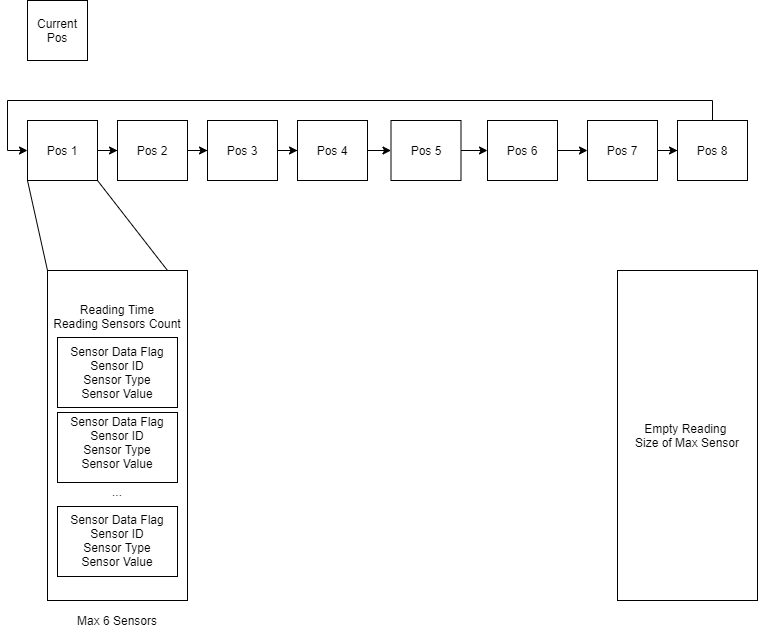
\includegraphics[width=0.80\textwidth]{images/circbuf.png}
\caption{Array Circular com leituras}\label{circbuf}
\end{figure}

\subsection {Sincronismo de leitura e envio} \label{sinc}

\par À semelhança dos restantes produtos produzidos pela Captemp, neste produto existe sempre sincronismo de leituras entre os equipamentos. Para tal além de cada equipamento possuir um relógio interno (RTC), é necessário fazer o sincronismo dos mesmos na primeira leitura. Isto é feito para evitar que, por exemplo um equipamento programado para fazer leituras a cada 5 minutos, que entre em funcionamento às 00h00, não faça leituras dessincronziadas com outro ligado às 00h12. Neste caso o primeiro equipamento fará leituras ao minuto 5, 10, 15, 20, enquanto que o segundo fará ao minuto 17 e 22.
\par Para tal o equipamento no momento inicial do arranque verifica qual o intervalo de leitura e de envio, e verifica caso fosse ligado pelas 00:00 qual seria a próxima leitura ao momento atual, neste momento o equipamento não entra em modo de poupança de energia durante os 5 minutos até á leitura e apenas o tempo restante até ao valor caso fosse ligado pelas 00:00, no momento da leitura o equipamento já entra em modo de poupança de energia durante o tempo definido (Ex:5 minutos). Este método é igualmente aplicado ao intervalo de envio. Aquando do envio é enviado na resposta proveniente do servidor o \textit{Timestamp} do servidor de modo a sincronizar o tempo de todos os equipamentos e configurar nos novos equipamentos que sejam ligados e ainda possuam o valor \textit{default} do RTC, no caso do escolhido no projeto 1 de Janeiro de 2000.
\par Caso o equipamento possuir uma data inferior á estipulada de 1 de Janeiro de 2019, o mesmo não faz leituras, esperando pelo intervalo de envio para enviar um pacote apenas com os campos fixos e sem leituras de modo a obter a resposta com o \textit{timestamp} do servidor para iniciar as leituras.


\subsection {Encriptação dos dados}

\par De modo a proteger os dados na rede todo o pacote é encriptado com recurso á biblioteca MicroPython-AES disponibilizada \textit{online} \cite{microaes}. Esta biblioteca foi desenvolvida para o MicroPython Base e não para a versão disponibilizada nos módulos DIGI. É necessário reformular a biblioteca do AES para MicroPyhton de modo a não utilizar a biblioteca de gestão de \textit{arrays} indisponível nesta versão. É necessário alterar a biblioteca para não usar as funcções da biblioteca de gestão de \textit{arrays} no momento que os dados são encriptados e desencriptados. No código \ref{py2} é apresentado o problema inerente a esta biblioteca (linha 4) e a sua respetiva resolução (linha 13 e 14).


\begin{lstlisting}[caption=Adaptação do Código para o equipamento Digi,label={py2},language=Python]
for offset in range(0, len(data), block_size):
    block = data[offset:offset + block_size]
    block_func(block)
    data[offset:offset + block_size] = block # ERROR 
    #['array' object does not support item assignment]
...

...
for offset in range(0, len(data), block_size):
    block = data[offset:offset + block_size]
    block_func(block)
    # Solution ['array' object does not support item assignment]
    for i in range(block_size)
        data[offset+i]= block[i]
 ...
\end{lstlisting}

\section {Kea Tracker}

\par De modo a substituir um produto descontinuado e apresentar novas soluções aos clientes, irão ser utilizados \textit{beacons} para armazenar os valores da temperatura, humidade e pressão ambiental para posterior envio para o portal Senslive. No início do estágio não estava disponível nenhuma versão de \textit{Firmware} com armazenamento dos dados e estava proposto o desenvolvimento da solução utilizando o Espruino, uma plataforma que permite fazer a programação de microcontroladores com recurso a JavaScript. Foram realizados pequenos testes e chegou-se à conclusão que a camada interpretadora do Javascript tem um consumo mais elevado comparando com uma versão desenvolvida em C. Além do maior consumo energético, já foi disponibilizado um \textit{Firmware} com armazenamento de leituras para posterior arquivo. Devido a esses dois fatores, não será desenvolvido o \textit{Firmware} como estava inicialmente proposto, mas em alternativa os esforços serão concentrados no melhoramento e desenvolvimento da aplicação responsável por obter os dados e enviar para o portal Senslive. 


\subsection{App - Alterarações necessárias}

\par A aplicação móvel na primeira fase irá ser baseada na fornecida pela Ruuvi e serão alteradas as referências ao \textit{website} da RuuviTag para o \textit{website} da Captemp e a alteração das imagens para o novo logótipo da solução. Devido é necessidade de desenvolvimento do \textit{Back-end} no Senslive, para já será adaptada apenas a versão Android da aplicação. Numa segunda fase do projecto, será desenvolvida uma aplicação para Android e iOS utilizando uma plataforma que permita o desenvolvimento para ambas as plataformas com apenas um código fonte, tais como o NativeScript\cite{nativescript}, o Ionic\cite{ionic} entre outras.

\subsection{App - Novas funcionalidades}

\par A aplicação fornecida pela Ruuvi não está desenvolvida para a consulta das leituras quando o \textit{beacon} não esteve ao alcance. É necessário então desenvolver o módulo por obter essas leituras e guardar na base de dados para a restante aplicação enviar para o portal Senslive.

\par O \textit{Firmware} disponibilizado converte a RuuviTag num \textit{beacon} connectável e disponibiliza sobre a forma de um serviço os Logs da mesma\cite{ruuvitlog}. Para tal é necessário adaptar a aplicação de modo a quando esta esteja encontra um novo \textit{beacon} ao alcance descarregue o seu Log. Quando o \textit{beacon} se encontra sempre ao alcance a aplicação não necessita de fazer a conexão para descarregar os Logs visto esta além da conexão faz o \textit{broadcast} dos dados em tempo real. O principal problema a resolver neste projeto é o sincronismo de leituras, já retratado no capítulo \ref{sinc} quando a aplicação se encontra a registar através do \textit{broadcast}. Nos Logs não é possível fazer esse sincronismo devido á mesma não possuir essa funcionalidade internamente. No \textit{download} dos Logs é necessário verificar quais as leituras de Log que possam ser referentes a intervalos que existiu a receção de \textit{broadcast} e tiveram leituras sincronizada, não sendo necessário o armazenamento. É espectável com o \textit{Firmware} selecionado obter uma autonomia entre 2 a 3 anos com ligações esporádicas para descarregar Logs ou 6 meses com a conexão sempre ativa. Nos Fluxogramas dos apêndices  \ref{E}, \ref{F} e \ref{G} é possível observar o ciclo referente á obtenção das leituras em tempo real para a atualização do dashboard, o descarregar dos Logs, o registo das leituras no intervalo definido e o envio para o portal também com sincronismo.

\par Sempre que a aplicação recebe uma nova transmissão cria um novo fluxo de processamento de modo a não congestionar a restante aplicação. É analisado a origem da transmissão e caso seja um dos \textit{beacons} registadas na aplicação esta é processada, em caso contrário é descartado. Caso seja uma transmissão de um \textit{beacon} que esteve fora de alcance num intervalo superior a 5 Minutos, corespondente ao intervalo de Log, é feito as tentativas de \textit{download} dos Logs, após esse \textit{downaload}é feito o processamento dos valores em tempo real presentes no pacote. 

\par Além dos valores em tempo real no dashboard são armazenados na memória RAM os valores referentes à última comunicação registada em cada minuto. Ao receber um pacote, caso este seja o primeiro do minuto da transmissão atual, isto é desde o segundo 0 do minuto esta é a primeira, então é registada como a leitura correspondente à do minuto atual. Caso já exista uma leitura desse minuto é atualizado apenas o \textit{dashboard} da aplicação. No minuto seguinte esta varíável é atualizada para a do minuto seguinte. Este proceso está representado no fluxograma do apêndice {G}.

\par Paralelamente à receção dos pacotes existem dois fluxos de processamento responsáveis por registar em memória não volátil as leituras a enviar e o envio das mesmas para o Portal. Seguindo o funcionamento de sincronismo de leituras já apresentado no capítulo \ref{sinc}, no intervalo correto é percorrido todos os \textit{beacons} é analizado a leitura sincronizada ao minuto e caso esta seja de uma data superior à ultima leitura é armazenada. Caso o \textit{beacon} tenha estado sempre ao alcance irá ser armazenada a leitura correta do minuto do registo definido nas configurações e criamos sincronismo entre registos dos vários equipamentos. Caso o \textit{beacon} tenha estado ao alcance mas no momento do registo sincronizado não se encontrava é guardada a última com a data/hora correspondente. Isto previne que, caso o \textit{beacon} não esteja ao alcance no minuto exato da leitura para sincronizar entre todas e caso tivesse estado ao alcance desde o último registo, exista pelos menos um registo a mostrar no gráfico apesar de este não estar sincronizado. De modo a todos os \textit{beacons} ao alcance comunicarem pelo menos uma vez no minuto do registo este processo é executado a cada intervalo de registo consoante o configurado mas com um atraso de 50s relativamente ao segundo 0 do minuto. Paralelamente a este fluxo existe o processo referente ao envio para o portal Senslive. Este também segue o mesmo principio de sincronismo de envio do capítulo \ref{sinc}. No apêndice \ref{E} e \ref{F} é possivel analizar o fluxograma referente ao processo de registo de leituras e do envio descrevido anteriormente.


% O principal problema deste projeto a resolver é a definição do intervalo que a aplicação deve descarregars os Logs da Beacon. No caso mais simples a aplicação num intervalo programado e fixo descarrega os Logs desde o ultimo \textit{download}, mas é criado um problema caso a beacon não esteja ao alcance no preciso momento do intervalo. Caso falhe um intervalo a beacon tem suporte para no intervalo seguinte descarregar ambos os intervalos, mas tem um limite, este variável consoante o valor definido como intervalo de \textit{download}. No caso apresentado anteriormente, no momento definido para descarregar os Logs a beacon pode não estar ao alcance, mas a mesma pode ter estado ao alcence momento antes ou momentos futuros. Nesses casos a aplicação deve segundo o tempo desde a ultima conecção verificar se a deve se ligar a beacon ou não diminuindo a possibilidade de perder leituras. Esta solução é necessário pois a beacon com o \textit{firmware} em questão caso esteja sempre com a connexão ativa para descarregar o Log da última leitura apenas tem autonomia para 6 meses e caso seja feito o \textit{download} periodicamente de um conjunto de Logs, uma autonomia espectável entre 2 e 3 anos. 

\subsubsection{\textit{Download} manual}
\par A aplicação desenvolvida permitirá ainda ao utilizador a possibilidade de fazer o \textit{download} dos Logs manualmente ao invés do \textit{download}, configurar o máximo de tentativas do \textit{download} automático, com o valor de \textit{default} definido em 1. Além dessa configuração é implementada uma medida de segurança onde caso o RSSI seja inferior a -90, significando que se encontra longe não são descarregados os Logs devido á possibilidade de perder a ligação no \textit{download}, neste caso é apresentado ao utilizador uma nota para aproximar o equipamento do \textit{beacon}. %Caso uma das beacons entre no alcance do Smartphone e a mesma tenha estabelecido a última ligação num intervalo superior ao configurado(\textit{default}- 1 Hora) a aplicação estabelecerá automaticamente a ligação para descarregar e minimizar a perda de leituras. Igualmente caso a beacon antes do intervalo definido esteja ao alcance e o sinal tenha um valor baixo, significando que se encontra longe e poderá não conseguir descarregar os dados a app descarrega os dados minimizando igualmente as perdas de possíveis dados.

\subsection{Desenvolvimento de uma aplicação multi-plataforma}

\par A \textit{Framework} escolhida foi o Ionic, uma \textit{Framework open-source} que permite o desenvolvimento de aplicações \textit{mobile} para múltiplas plataformas com o mesmo código, diminuindo o esforço necessário para o desenvolvimento e simplificando os processos de atualização visto apenas existir um código fonte a atualizar. 

\par Esta fase do projeto Kea.Tracker é referente à conversão da aplicação existente em Kotlin para o Ionic e migrar todas a funcionalidades existentes atualmente na versão em Kotlin. 
Ao invés da utilização de \textit{Activities} como no Kotlin o Ionic utiliza um sistema similar a um serviço WEB onde são criadas várias rotas e é possível navegar entre elas. Todo o \textit{design} da plataforma seguiu o mesmo layout da aplicação já existente, onde foram retiradas as opções de alertas e vizualização dos gráficos visto pretendermos centralizar essas opções no portal Senslive e utilizar a aplicação apenas como um \textit{Gateway}. Fica assim disponível na aplicação apenas a opção de adicionar novos equipamentos ao gateway neste caso à App, editar o nome do equipamento para mais fácil distinção entre os vários equipamentos, as configurações da aplicação e um serviço em \textit{Background} para realizar as leituras sem necessidade da aplicação estar aberta.
	
\subsubsection{Distinção entre \textit{Beacons} \& Leitura de Dados  }

\par Para facilitar a utilização da interface da aplicação ao utilizador da mesma, ao adicionar um novo dispositivo apenas são mostrados os dispositivos ao alcance que correspondam a equipamentos da Ruuvi e que estejam a transmitir os dados nos formatos definidos. Todos os equipamentos BLE possuem nos dados transmitidos por \textit{Broadcast} possuem primeiro informações no \textit{header} da transmissão, tais como o fabricante, denominado de \textit{"Company Identifier"}. No caso dos \textit{beacons} da Ruuvi é enviado o código  correspondente à Ruuvi, "0x0499". Estes códigos podem ser consultados na documentação do \textit{Bluetooth} \cite{companySI}. Juntamente com o \textit{Company Identifier} o protocolo define mais alguns parâmetros tais como o tamanho do cabeçalho. No caso dos \textit{beacons} da Ruuvi são enviados os dados referentes aos sensores nos diversos formatos definidos na documentação da Ruuvi \cite{GitHubRuuvi}, precedidos por um byte com o valor correspondente  ao formato dos dados.
\par Segundo a documentação a aplicação deve suportar a leitura em tempo real de dois formato o formato 3 e 5, pois são estes os existentes nos \textit{beacons} atuais em produção.



\section {dot.Tracker}
\par
A pedido de um cliente, foi proposto o desenvolvimento de uma plataforma WEB para fazer a monitorização de pessoas e objetos em tempo real. O projeto passou por várias etapas das quais destacam-se a análise dos requisitos do cliente, análise de tecnologias disponíveis, análise de soluções existentes já em comercialização, o desenvolvimento do portal Web, desenvolvimento do Back-End, e testes ao sistema. Apesar do projeto ser apenas desenvolvido por um elemento, mas devido á maior complexidade e duração do mesmo foi adotada a metodologia SCRUM com entregas/apresentações ao cliente para obter o \textit{feedback} do trabalho desenvolvido e assim poder alterar alguns dos requisitos solicitados.
\par O Cliente indicou que devia ter atualizações dos mapas em tempo real, alertas enviados para o cliente WEB caso este esteja \textit{online} e por email.
É assim possível definir a tabela, apresentada na tabela \ref{tab1} com os requisitos da solução e a sua importância no desenvolvimento.

\begin{table}[htb]
\centering
\caption{Requisitos da solução}\label{tab1}
\begin{tabular}{|p{3cm}|p{8cm}|p{2cm}|}\hline
Requisito&Descrição&Importância (1-10)\\\hline

Portal Cloud (Front-End)&Portal Cloud com mapas em tempo Real& 7\\\hline
Portal Cloud (Back-End) & API REST para integração com o Front-End e recolha dos dados para a localização &9\\\hline
Histórico de posições&Possibilidade de re-visualizar no mapa o percurso entre datas&5\\\hline
Alertas Email&Alertas de Email (Exemplo: Entrada e Saída de zonas criadas no mapa )&6\\\hline
Alertas Web&Alertas Informativos no Mapa (Exemplo: Entrada e Saída de zonas criadas no mapa )&2\\\hline
\end{tabular} 
\end{table}

\par
De seguida são apresentados as funcionalidades e objetivos para cada módulo do projeto \textit{Front-end} e \textit {Back-end}.

\subsection {Portal Cloud - \textit{Front-End}}

\par O \textit{Front-end} da solução é desenvolvido com recurso á \textit{Framework Vue}, tornando a solução numa solução \textit{Single-Page Aplication}. A adoção da \textit{framework} é baseada na necessidade de possuir fluidez na navegação entre páginas e igualmente nos mapas em tempo real minimizando o atraso.
\par A plataforma é capaz igualmente de suportar várias \textit{Companies}, significa isto que é possível criar várias organizações ou empresas distintas (\textit{Companies}) e temos os administradores e os utilizadores normais de cada \textit{Company} que apenas tem acesso ás suas definições e equipamentos. Possibilitando fornecer o projeto como uma solução \textit{Cloud} a váriados clientes no mesmo servidor, onde cada um apenas possui o acesso ao que pertence à sua \textit{Company}.
No final o utilizador da plataforma deve ser capaz de realizar as seguintes operações:
\par
\begin{itemize}
\item Login na plataforma para visualizar os dados
\item Visualizar mapas com atualizações em tempo real
\item Editar o seu perfil
\item Visualizar a página numa língua á sua escolha
\item Utilizar a plataforma em vários equipamentos PC, Tablet, Smartphone,...
\item Gerir utilizadores (Administradores)
\item Gerir equipamentos (Administradores)
\item Gerir mapas e zonas (Administradores)
\item Gerir alertas (Administradores)
\item Iniciar/ finalizar missões (Administradores)
\end{itemize}


\subsubsection{\textit{Login}}
\par Para aceder á plataforma é necessário aos utilizadores procederem ao login na mesma, uma vez que possuímos uma API o \textit{login} é realizado através de Json WebTokens ou simplesmente, JWT. No momento do \textit{login} são enviadas as credenciais para o servidor, caso este as valide cria um \textit{Token} que é devolvido ao cliente e este em futuras requisições à API inclui o \textit{token} identificando-se e autenticando-se perante o servidor. Este método de login é regularmente utilizado devido á necessidade de possuir métodos \textit{stateless} ao invés da utilização de variáveis de sessão. No exemplo apresentado na figura \ref{jwt1} é apresentado o conteúdo de um \textit{Token} JWT. 


\begin{figure}[ht]
\centering
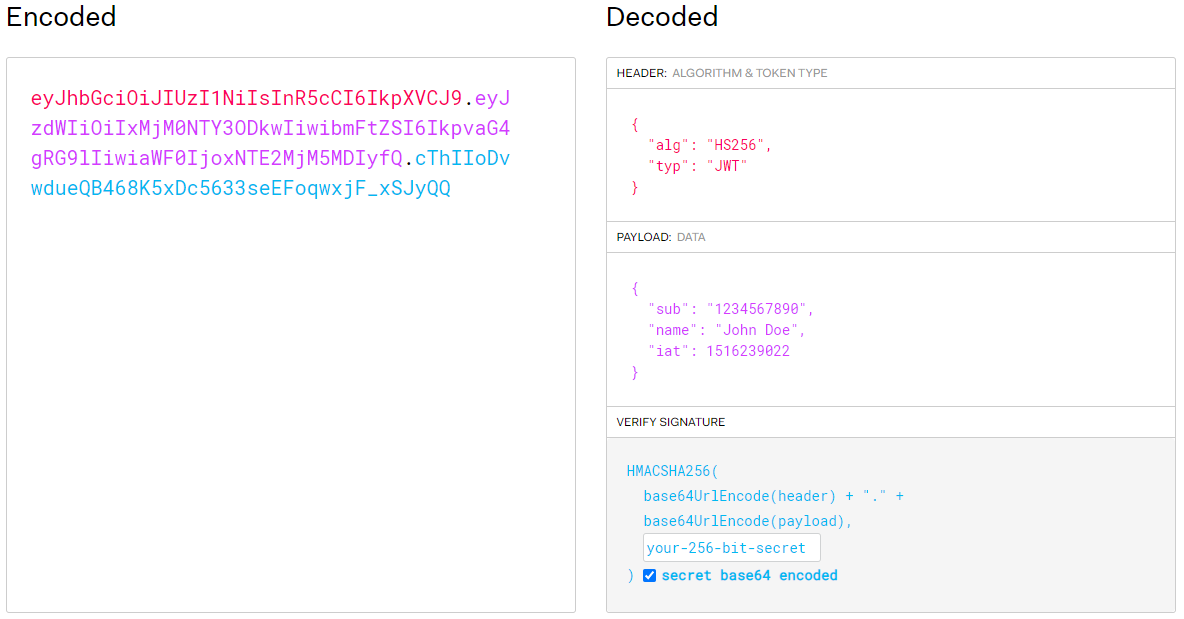
\includegraphics[width=0.85\textwidth]{images/jwt.png}
\caption{Token JWT codificado e descodificado \cite{jwt}}\label{jwt1}
\end{figure}

\subsubsection{Rotas e proteções}

\par Para proteger as páginas apenas referentes a administradores e as gerais ao público não autenticado através da \textit{framework Vue} e da funcionalidade de rotas foram criadas as rotas necessárias para o funcionamento da plataforma e os restantes \textit{end-points} são tratados por uma vista de erro indicando ao utilizador que não existe aquele \textit{end-point}. Em cada rota é aplicado um \textit{middleware} para verificar as permissões. Os \textit{middlewares} criados verificam se o utilizador está autenticado e no caso de serem necessárias permissões se este as possui ou não. Caso o \textit{middleware} indique que não tem acesso a \textit{framework Vue}, redireciona para a rota de tratamento de erro apresentado a mensagem de erro correspondente.

\subsection{Portal Cloud - \textit{Back-end}}

\par O \textit{Back-End} é responsável por fornecer uma API REST ao \textit{Front-end} para o mesmo obter os dados da base de dados. É igualmente responsável por obter os dados provenientes dos \textit{Gateways} dos \textit{beacons} e calcular as suas posições para apresentar no mapa. 

\par O primeiro problema identificado no \textit{Back-end} é a necessidade de possuir atualizações em tempo real das posições. O \textit{Front-end} não é capaz de calcular quando um \textit{beacon} comunica com o \textit{Back-end} apesar do mesmo enviar o \textit{broadcast} em tempos regulares, mas tanto o \textit{beacon} pode não estar ao alcance do \textit{Gateway}, como o mesmo pode apenas estar ao alcance de menos de X(dependendo do algoritmo) \textit{Gateways} impossibilitando a utilização do algoritmo. Deste modo não é eficaz o \textit{browser} solicitar ao servidor num intervalo regular qual a posição do elemento no mapa.

\par Para tal além do serviço WEB é disponibilizado um servidor de WEB-Sockets para comunicações em tempo real entre o \textit{Back-end} e o \textit{Front-End}. Os WEB-Sockets são uma tecnologia que permite aos \textit{browsers} mais recentes, ter um canal em tempo real com o \textit{Back-end} sem a necessidade de fazer vários pedidos HTTP, o que acarreta todo o processo do protocolo, como o \textit{3-Way Handshake}. No momento da criação do Web-Socket é criado uma ligação TCP a qual não é finalizada até ao fechar do WEB-Socket, o que elemina o sobre carregamento da criação de pedidos e soluciona o problema da comunicação em tempo real para as atualizações dos mapas.

\par Outro problema a solucionar, identificado na análise das tecnologias e soluções existentes, é a falta de sincronismo da comunicação dos \textit{Gateways}. Supondo um cenário com 5 \textit{Gateways} e 1 beacon. O \textit{beacon} ao intervalo de tempo X1 comunica o pacote e apenas 4 \textit{Gateways} recebem o pacote e o enviam para o servidor através de um pedido HTTP. O servidor apesar de ter configurado 5 \textit{Gateways} não é capaz de prever se o 5º \textit{Gateway} irá comunicar a transmissão do \textit{beacon}, o mesmo pode não estar ao alcance, pode não ter comunicação ao servidor, pode estar desligado ou pode haver algum problema na rede que atrase a chegada do pacote. Igualmente por variados motivos os 4 \textit{Gateways} que enviaram o pacote ao servidor não irão chegar todos em simultaneamente, criando o problema "Já chegaram todos os pacotes? Cálculo com os que tenho, ou espero que chegue mais algum pacote?",

\par A primeira solução adotada para resolver o problema acima citado foi, ao contrário da utilização de servidores WEB como o APACHE2 ou NGINX comuns nas soluções tradicionais a utilização de Node.js (módulo express). 
\par As soluções tradicionais não possuem nenhum sincronismo entre pedidos, isto é, não é possivel aceder diretamente ao valor existente no fluxo de um outro pedido e seria necessário armazenar momentaneamente todos os pacotes na base de dados e ter a tabela em constante escrita e leitura, não sendo o mais eficaz no cenário deste projeto. Na solução desenvolvida, é possível armazenar variáveis entre pedidos distintos e irá ter além do serviço WEB o servidor de WEB-Sockets no mesmo processo, centralizando assim os dois serviços e possibilitando igualmente durante o processamento do pedido HTTP o envio de mensagens através do WEB-Socket. 
\par O módulo express é uma \textit{Framework} desenvolvida para Node.js para aplicações que necessitam de rapidez de resposta nos pedidos e á semelhança de outras \textit{frameworks} em outras linguagens permite a utilização de rotas para a criação dos \textit{end-points}.
\par Na lista apresentada de seguida estão selecionados os pontos principais das funcionalidades do \textit{Back-End}:

\par
\begin{itemize}
\item API REST para o \textit{Front-End}(Login+ Dados)
\item API REST para o POST dos \textit{Gateways}
\item Serviço WEB (express) para disponibilizar o \textit{Front-End}
\item Serviço WEB-Sockets 
\item Algoritmo de posicionamento
\item Envio de alertas
\end{itemize}
\par

\subsubsection{Sincronismo da receção de pacotes}
\par Os \textit{Gateways} escolhidos enviam dois tipos de pacotes identificados pelos identificadores GPRP e RSPR. Os pacotes GPRP são referentes ao envio de uma transmissão do \textit{beacon}. Os pacotes RSPR são referentes ao restante da transmissão do \textit{beacon} no caso de esta transmitir no Broadcast uma mensagem superior a 31 bytes. O conteúdo do pacote RSPR apenas contem o restante da mensagem não afetando a posição do \textit{beacon}.
\par De modo ao servidor possuir todos os pacotes GPRP aquando da utilização no momento da chegada este é armazenado numa variável onde é possível consultar as ultimas transmissões de todos os \textit{Gateways}. Quando é recebida uma transmissão do tipo GPRP caso esta seja enviada do \textit{Gateway} X e a ultima transmissão do \textit{Gateway} X for inferior a 5 segundos (intervalo de envio do \textit{beacon}) este mesmo pacote é descartado, pois o mesmo é referente a um já recebido. Caso seja superior aos 5 segundos do próprio \textit{Gateway} e de todos os restantes, significa que a mesma se trata de uma nova transmissão, neste caso antes de guardar na variável provisória, são selecionados todos os pacotes do intervalo correspondente á ultima transmissão e escolhidos os 4 com o valor mais próximo dos \textit{Gateway}, devido a estes serem os mais fiáveis e é aplicado o algoritmo \textit{Least Squares Estimation} ou simplesmente LSE. Após obtenção da posição estimada esta é guardada na Base de dados para consulta futura e são notificados os clientes de uma nova posição do equipamento. Caso essa posição seja referente a alguma zona de alertas previamente definida é gerado os alertas a enviar. No fluxograma do Apêndice \ref{flux1} é apresentado o fluxograma da aplicação para a receção dos pacotes.


\subsubsection{Diferenças de alturas}

\par Uma questão analisada nos primeiros testes é a divergência nas distâncias observadas quando o \textit{beacon} apenas se movia no eixo do Z (altura). O \textit{Gateway} calcula a potência do sinal(RSSI) recebido do \textit{beacon}, esta receção ocorreu em linha reta entre os dois equipamentos e nos mapas utilizados apenas são utilizadas dimensões 2D significando que o valor da distância obtido pelo RSSI é referente ao mesmo em linha reta e não á distancia numa planta 2D, como é apresentado na figura \ref{altura1}.

\begin{figure}[ht]
\centering
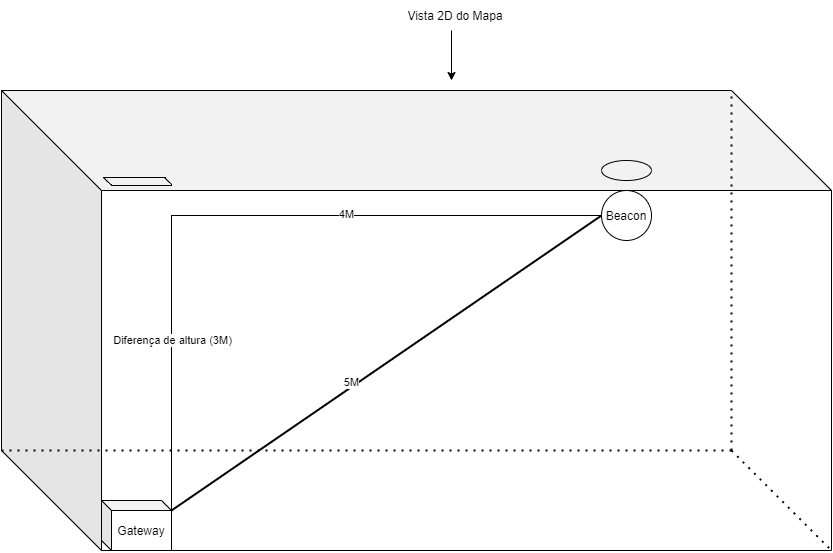
\includegraphics[width=0.95\textwidth]{images/disr.png}
\caption{Diferença entre distâncias Planta vs realidade}\label{altura1}
\end{figure}


\par Para tal na aplicação teve de ser desenvolvido a possibilidade de o utilizador configurar as alturas a que se encontram os \textit{Gateways} e ps \textit{beacons}, de modo a compensar a distância. No exemplo apresentado na figura \ref{altura1} o servidor irá receber a informação que o \textit{Gateway} recebe um pacote com o RSSI correspondente á distância de 5 metros mas no mapa não é a distância a considerar para utilizar o algoritmo que apenas possui suporte a coordenadas 2D. Para tal é necessário conjugar a diferença de alturas e a distância em linha reta para calcular a distância a considerar para o algoritmo, segundo o teorema de Pitágoras. No caso exemplificado ao invés dos 5 metros deve ser considerado os 4 metros.

\subsubsection{Algoritmo de triangulação}

\par Para o projeto foi selecionado o Algoritmo LSE analisado no Capítulo \ref{indoor}, pois o mesmo demonstra os melhores resultados em vários testes. Como parâmetros deste algoritmo é necessário indicar as posições X,Y de cada \textit{Gateway} e a distância calculada previamente segundo o RSSI e o algoritmo de Pitágoras de modo a resolver a diferença referente á altura.

\par No Caso do mapa ter configurado um número superior ao necessário para a utilização do algoritmo, neste caso 4, e nos casos em que existam mais do 4 \textit{Gateways} que receberam comunicações apenas são utilizadas as 4 que tiverem menores valores de distância, visto que estando mais próximas o algoritmo não tem um erro tão elevado. Previamente à seleção das 4 melhores transmissões caso alguma das transmissões tenha uma distância inferior a 1 metro não é utilizado o algoritmo e é definido a posição do \textit{beacon} igual à posição do \textit{Gateway} no mapa. Caso não exista nenhum valor abaixo do 1 metro é utilizado o algoritmo indicado.
 
\par De modo a otimizar o processamento do algoritmo, devido a este envolver cálculos em matrizes e estas não possuírem tamanhos dinâmicos, não foi utilizada nenhuma biblioteca para realizar as operações em matrizes devido ao peso computacional excessivo que estas apresentam. Ao invés, as operações sobre matrizes foram implementadas manualmente conforme as  necessidades do projecto, usando as regras de operações. Cada variável possui o valor de uma posição da matriz correspondente. No apêndice \ref{D} é fornecida a função responsável por retornar a posição estimada do \textit{beacon} ou -1 em caso de erro ou o mapa definido não possua a escala definida, apesar da plataforma não permitir adicionar \textit{Gateways} a mapas sem escala. No caso especifico apresentado nas linhas 47 a 50, de modo a otimizar a eficiência do algoritmo, é efetuada a multiplicação por 0.5 em vez da divisão por 2, uma vez que esta é computacionalmente mais eficiente.
\subsubsection{Filtros - RSSI}

\par Após o desenvolvimento do algoritmo e de alguns testes à receção de pacotes, foi possível verificar que, numa sala com 6 metros analisar numa sala com 36 metros quadrados e 4 \textit{Gateways} e com 4 Gateways, o sinal dos \textit{beacons}, colocadas em posições fixas (estratégicas), sofre de algumas flutuações, fazendo com que o algoritmo devolva posições incorrectas. De modo a eliminar essas flutuações é necessário filtrar os pacotes com ruido e tentar aproximar o valor do esperado. Para tal irá ser utilizado um modelo matemático denominado por Filtro de \textit{Kalman}\cite{KalmanFilter2}. Este modelo matemático é capaz de ao longo do tempo consonante os valores recebidos tentar aproximar o valor recebido do espectável segundo a tendência anterior. Deste modo é necessário alterar o servidor de modo a além de guardar temporariamente os pacotes inserir o valor no filtro correspondente. Por cada \textit{beacon} existente na plataforma existe um conjunto de filtros, um por cada \textit{Gateway} que já recebeu alguma comunicação do \textit{beacon}. Sempre que um \textit{Gateway} comunica a receção de um pacote do \textit{beacon} o valor recebido do RSSI é inserido no filtro onde é retornado o valor estimado segundo os valores anteriormente recebidos. No exemplo da figura \ref{kalman1} é possível observar o funcionamento do filtro ao longo do tempo. Para o projeto é utilizado o plugin JavaScript\cite{kalman} disponível no GitHub onde é implementado o filtro \textit{Kalman} para dados do tipo 1D. Um dos fatores para a utilização deste filtro ao invés de outros, além da sua utilização por parte de outras pessoas na comunidade científica no âmbito das localizações \textit{inndoor}, foi a necessidade de um algoritmo rápido a estabilizar os dados e que não sobrecarregue o servidor. Após analise do filtro foi possível analisar, que por cada filtro apenas são alojados em memória o último valor e 6 variáveis referente aos cálculos necessários na próxima filtragem, não sendo o espaço assim influenciado pelo tempo que tiver em funcionamento.

\begin{figure}[ht]
\centering
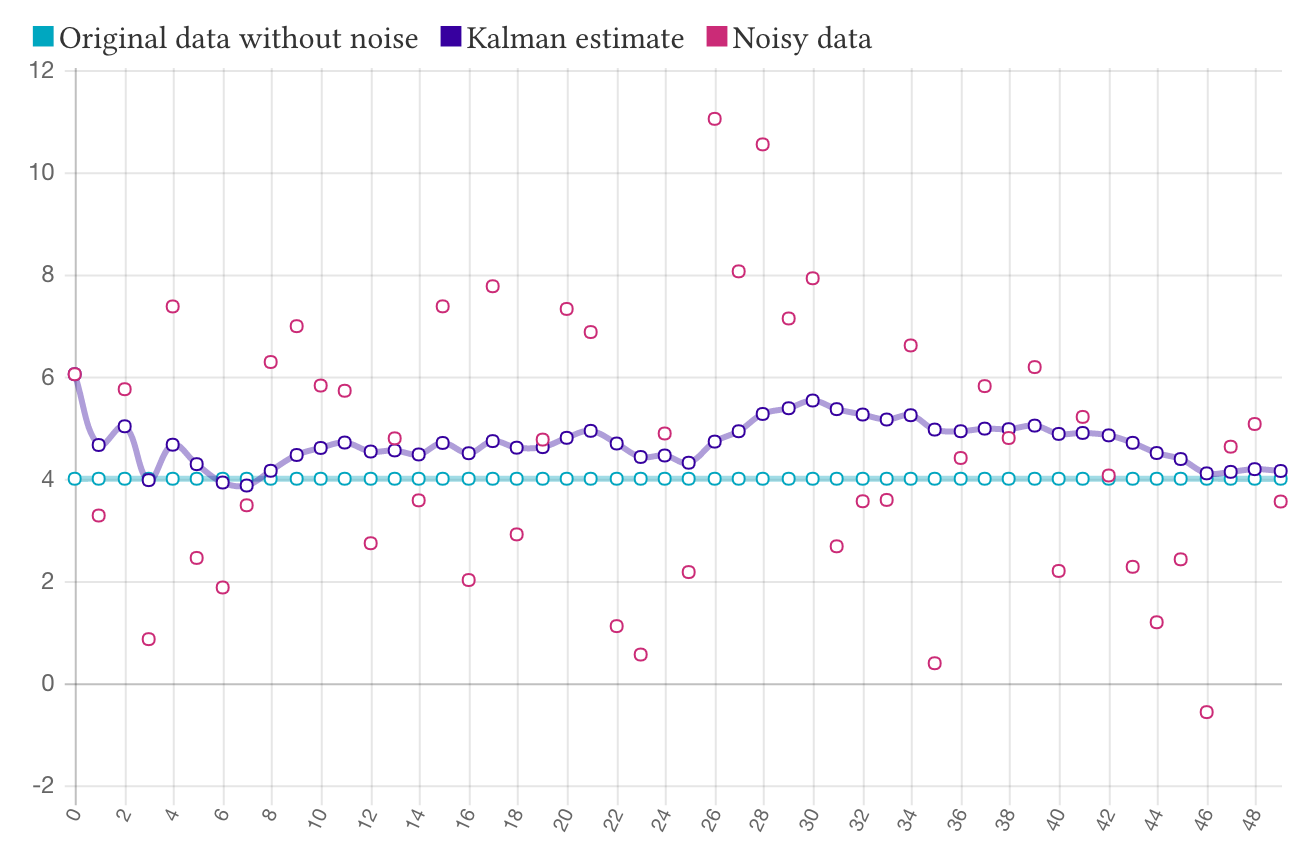
\includegraphics[width=0.90\textwidth]{images/kalman-example.png}
\caption{Exemplo da aplicação do Filtro Kalman \cite{kalman}}\label{kalman1}
\end{figure}



\subsubsection{Filtros - Posição no mapa}

\par Após filtragem do ruido gerado pela transmissão dos dados no meio ambiente, é necessário ainda filtrar certas ocorrências que ocorrem em certas posições e suavizar o movimento quando os \textit{beacons} se encontram em movimento. O primeiro caso a filtrar referente ao caso do \textit{beacon} esteja numa posição X1,Y1 no momento t e no momento t+1 em X2,Y2 onde a distância entre pontos é elevada. Para tal, quando uma posição é calculada segundo o algoritmo LSE, esta posição é comparada com a última guardada do mapa correspondente e é calculada a distância entre ambos os pontos, de seguida é calculada igualmente a velocidade segundo o tempo entre as leituras e a distância. Caso esta seja superior à definida, 5 m/s (18 Km/h), esta posição não é considerada enquanto o tempo entre leituras não permitir o deslocamento da pessoa/objeto para essa mesma posição. O valor máximo da velocidade é possível de ser adaptado consoante o pretendido medir, mas neste caso o cliente pretende monitorar pessoas e objetos. Os objetos alojados no armazém devem ter um deslocamento maioritariamente de 0 pois encontram-se parados e o valor de 5m/s corresponde á possibilidade de estar em movimento num empilhador ou similar. A velocidade média de uma pessoa a andar é de cerca 1 a 2m/s em caminhada\cite{walkingSpeed} e cerca de 1 a 3.8m/s \cite{Long2013}. em corrida, valores sempre inferiores à já definida no intervalo dos objetos.
\par Outro filtro a aplicar é no caso particular de um \textit{beacon} se encontrar parada e apesar do filtro \textit{Kalman} filtrar o RSSI a posição possuir pequenas oscilações. Para tal, se for gerada uma nova posição, esta tem de passar no filtro da velocidade pois se esta encontrar-se parada e perto da posição da última comunicação com pequenas oscilações e esta oscilação for inferior a 1 metro a posição é guardada mas não é enviada nehuma notificação para ser atualizada nos mapas através do Web-Socket. Na próxima receção caso esteja numa posição inferior a 1 metro da posição do mapa dos \textit{browsers} e a menos de 1 metro da ultima posição guardada existente apenas no servidor, não é atualizada a posição apenas novamente no servidor para futura comparação, caso não aconteça e esteja a menos de 1 metro da ultima guardada no servidor e a mais de 1 metro da presente nos \textit{browsers} esta é guardada e enviada para os \textit{browsers} através do Web-Socket. Caso se encontre a uma distância superior a 1 metro em ambas e abaixo dos 5m/s a posição é atualizada no servidor e nos \textit{browsers}.

\subsubsection{Zonas de alerta}

\par Um dos requisitos do cliente na solução é a definição de zonas de alerta, onde é possível indicar se a plataforma deve enviar alertas quando os \textit{beacons} saem ou entram de uma zona. Para a criação de uma zona de alerta no \textit{Front-end} é necessário o utilizador definir os vários vértices da zona no mapa selecionado. Após a definição da regra e dos limites, é necessário que, durante o cálculo de uma posição, o servidor verifica se o \textit{beacon} saiu ou entrou numa zona definida como alarme. No caso de polígonos regulares tais como círculos, retângulos, triângulos é facilmente calculado se um ponto se encontra dentro da área. No caso de polígonos irregulares o caso é diferente. Para tal foi utilizado na solução o plugin "point-in-polygon" \cite {pointpoint}. Este algoritmo é capaz de indicar se um determinado ponto X,Y se encontra dentro do polígono ou fora, definido pelos conjunto de pontos fornecidos .

\subsection{Reutilização de beacons}

\par De modo a construir uma plataforma modular e reutilizável, cada \textit{beacon} pode ser reutilizada na plataforma. No momento da configuração é adicionada um \textit{beacon} à conta da organização. Para as posições serem guardadas na base de dados é necessário o utilizador aceder à plataforma e iniciar uma missão indicando a data de início, se pretende localizar pessoas ou objetos e qual o utilizador/objeto a localizar. Neste momento sempre que o \textit{beacon} seja localizada nos mapas referentes à organização detentora do \textit{beacon} a posição é guardada com informação sobre a missão do \textit{tracking}. Quando o \textit{beacon} já não é necessária o utilizador pode terminar a missão do \textit{beacon} e a plataforma deixa de registar as posições enquanto não possuir missão ativa novamente. Desta forma o cliente pode adquirir vários \textit{beacons}, mas caso pretenda mudar de objetivo, como por exemplo um empregado deixe de trabalhar na empresa e começar outro funcionário pode ser trespassada o \textit{beacon} e nos históricos estes ficam separados e é possível de forma intuitiva decidir quais os dados que são de cada utilizador, excluindo a necessidade de utilizar um \textit{beacon} com um identificador diferente (MAC) para isso.
\par
